% !TeX spellcheck = en_US

%\PassOptionsToClass{peerreview}{IEEEtran}

\documentclass[acmsmall, screen, review]{acmart}

\usepackage{natbib}

\acmJournal{TOPS}


% *** GRAPHICS RELATED PACKAGES ***
%
%usepackage[pdftex,final]{graphicx}
%\graphicspath{{./inc/}{../../inc/}{./jpeg/}}
%\DeclareGraphicsExtensions{.pdf,.jpeg,.png}

% *** MATH PACKAGES ***
%
\usepackage{amsmath}
\microtypesetup{expansion=false}

% *** ALIGNMENT PACKAGES ***
%
\usepackage{array}

% correct bad hyphenation here
\hyphenation{ana-ly-sis Wiki-Leaks}

%%%%%%%%%%%%%%%%%%%%%%%%%%%%%%%%%%%%%%%%%%%%%%%%%%%%%%%%%%%%
%% Custom Packages not from the template
%%%%%%%%%%%%%%%%%%%%%%%%%%%%%%%%%%%%%%%%%%%%%%%%%%%%%%%%%%%%
\usepackage{nth}
%\usepackage[hidelinks]{hyperref}

% Document annotations
\usepackage[nomargin,draft]{fixme}
\fxsetup{layout=pdfnote}

\usepackage{fixfoot}


\begin{document}

\title{Unobservable Messaging with MessageVortex}

\author{Martin~Gwerder}
\orcid{0000-0003-0296-5079}
\affiliation{
	\institution{University of Applied Sciences Northwestern Switzerland}
	\city{Windisch}
	\state{AG}
	\country{Switzerland}
}
\affiliation{
	\institution{University of Basel}
	\city{Basel}
	\state{BS}
	\country{Switzerland}
}
\email{martin.gwerder@fhnw.ch}

\acmSubmissionID{0} % FIXME if we get a nuber from the submission system


\begin{abstract}
In this paper, we introduce an unobservable, censorship-resistant message anonymization protocol, named MessageVortex. It bases on the zero trust principle and a distributed peer-to-peer like architecture and avoids central aspects such as fixed infrastructures within a global network. Instead of using traditional aproaches like creating a new layer 3+ protocol, we blend our its traffic into suitable existing transport protocols, thus, making it next to impossible to block traffic with traditional means such as firewalls, without significantly affecting regular users of the transport medium. The protocol requires no additional protocol-specific infrastructure in public networks and allows a sender to control all aspects of a message such as the degree of anonymity, timing, and redundancy of the message transport without disclosing any of these details to the routing or transporting nodes. 
\end{abstract}

\maketitle

\section{Introduction\label{sec:introduction}}
Networks build a base of our communication-based society these days and allow us to connect quickly with any person or company of our wish. At the same time they allow to collect vast amounts of data. Such collected data may be used to judge upon our intentions and, therefore, this data is not only confidential, if we have something to hide. This problem has dramatically increased in the last years as big companies and countries started to collect all kinds of data and created the means to process them. Such a judgment allows, supposedly, to classify people and their intentions. This judgment is not limited to what they are doing but as well, on what they did and what they might do. Numerous events, present and past, show that multiple actors, some of which are state-sponsored, collected data on a broad base within the Internet. Whether this is a problem or not may be disputable. Undisputed is that such data requires careful handling, and accusations should then base on solid facts. Unacceptable seems the use of ``guesses'' or ``extrapolations'' in most of the cases. This may happen even under complete democratic control \cite{Leuenberger1989}.

Whistleblower Edward Snowden leaked a vast amount of documents. These documents suggested that such attacks on privacy commonly exist on a global scale. According to these documents, the National Security Agency (NSA) infiltrated tentousands of computer networks with malware to collect classified or personal information. They furthermore infiltrated Telecom-Operators such as Belgacom to collect data and targeted high member of governments even in associated states \cite{NCR2013,XKeyscore,Ball2013,Ackerman2013,Greenberg2013}. The magnitude of these programs are vast. XKeyscore spanned (in 2008) $\approx150$ sites with $700$ Severs collecting emails, web traffic, and chat messages.

Collection of vast amounts of data allows a potent adversary to build a  profile of a person. Unlike in the past, the availability of this information rose to new heights with the Internet. An entity in possession of such Profiles may use them for many purposes. These include service adoption, directed advertising, or classification of citizens. The examples given above show that the effects of this data is not limited to the Internet but reaches us effectively in the real world. While directed advertising may be classified as legit use, a general classification of citizens was considered as unacceptable in the past (see previously quoted documents \cite{NCR2013}, \cite{XKeyscore}, \cite{Ball2013}, \cite{Greenberg2013},\cite{Leuenberger1989}).

The main problem of this data is that it may be collected over a considerable amount of time and evaluated at any time. It even happened that standard practices of the time are judged differently upon later. Persons may then be judged retrospectively upon these types of practice. This questionable type of judgment is visible in the tax avoidance discussion\cite{Amat1999}. 

This list of events shows that big players are collecting and storing vast amounts of data for analysis. The list of events also shows that the use of this data has in the past been at least partially questionable. A lot of communication today is unencrypted (e.g., email) and a valuable source of knowledge. But not only the message content is important. Metadata such as message sizes, peer partners, message size, or suspected properties of peer partners are used in Social Network Analysis. According to \cite{Ackerman2013}, NSA uses such methods to identify potential terrorists. A suitable anonymity protocol has, therefore, not only to hide a message but additional attributes as well. It includes, leaving the message itself aside, all metadata, and all the traffic flows. As a part of possible countermeasures, this work analyses the possibility of using state-of-the-art technology for messaging to minimize the information footprint of a person on the Internet. It should be censorship-resistant, having no specific or centralistic infrastructure making it possible to pressurize owners or maintainers. 

Our work tries to fill the gap and provides an unobservable and under ideal conditions censorship-resistant protocol called \emph{MessageVortex}. It combines well proven technologies such as F5 steganography and onionized routing structure. MessageVortex has been developed and published as RFC-draft. Furthermore, an implementation for academic research exists. 

To be censorship-resistant \emph{MessageVortex} features some unique properties. First there is no protocol specific infrastructure in the internet required. The protocol pigibacks common messaging protocols such as SMTP or XMPP. This means that ordinary account of messaging providers (such as freenet, gmx, gmail, or yandex) may be used as infrastructure. The messages themselfes are kept as undistinguishable as possible from regular messaging traffic. Only an endpoints blending layer residing on a endpoint device is able to tell if am message contains traffic destined for the current node of the \emph{MessageVortex} network. All endpoint devices (e.g., smartphones or notebooks) work alike and there are no such things as entry or exit nodes as there are in other similar systems such as ToR\cite{tor-spec}. Central infrastructure such as keyservers, directory servers or similar does not exist. This lack makes the protocol less susceptible to attacks.

The messages themselfes are routed in an onionized form. Unlike in compareable systems, the message is not routed as a whole or in a chunked form. Instead the routing information contains instructions about how to handle all parts of the message. The instructions are crafted in such a way that an attacker is unable to distinguish decoy from payload traffic even if having a full insight into a routing node.

MessageVortex does not rely on the trust of infrastructure other than the infrastructure under control of the sending or receiving entity. Trust in any third party might be misleading in terms of security of the protocol. Central infrastructure is bound to be of particular interest to anyone gathering data. It may furthermore allow manipulating the system or the data or the data flow. Therefore MessageVortex does not have such infrastructure. The only protocol specific devices are the endpoint devices of the users.

A problem of such mass surveillance is the possibility of censorship. For censorship, we take a definition attributed to Chuck Stone, professor at the School of Journalism and Mass Communication, University of North Carolina. 
\begin{quote}
	Censorship: the cyclical suppression, banning, expurgation, or editing by an individual, institution, group or government that enforce or influence its decision against members of the public -- of any written or pictorial materials which that individual, institution, group or government deems obscene and ``utterly without redeeming social value,'' as determined by ``contemporary community standards.''
\end{quote}

Please note that ``Self Censorship'' (not expressing something in fear of consequences)  is a form of censorship according to this definition too. In our technical context, we reduce the definition to
\begin{quote}
	Censorship: A systematic suppression, modification, or banning of data in a network by either removal, or modification of the data, or systematic influencing of entities (e.g., servers, networks, or operators) involved in the processing of this data.
\end{quote}
This simplified definition narrows down the location to computer networks.  Furthermore, it limits the definition to the maximum reach within that system. A censorship-resistant system is a system which allows the entities of the system and the data itself to be unaffected from censorship. Please note that this does not deny the presence of censorship per se. It still may exist outside the system or may be ineffective within the system. 

In consequence, people must be able to control their data footprint. Not providing this possibility does effectively allow any country or a bigger player to ban and control any number of persons within or outside the Internet.  

In the next section, We explain roughly the main characteristics and working of our protocol mitigating these problems. We then introduce some of the core terms and a general adversary model. We furthermore elaborate on the Notation used to describe our protocol. In section \ref{sec:protocol}, we dive into the technical details of the protocol and describe its operations in detail. In section \ref{sec:discussion}, we discuss some of the key findings related to the protocol.

\subsection{Formalization}
\subsubsection{What We Worked On}
In this work, a new protocol is designed to allow message transfer through existing communication channels. These messages are next to unobservable for any third party. This unobservability does covers the message and all metadata and flows associated with it. We called this protocol ``MessageVortex''. The protocol is designed to be capable of using a wide variety of transport protocols. It is possible to switch protocols while the messages are transferred. This behavior allows media breaches on a protocol level and makes an analysis of the message flow for any adversary harder as analysis have to span multiple protocols. MessageVortex allows secure communication without the need for trusting the underlying transport media. Furthermore, the usage of the protocol itself is possible without altering the immediate behavior of the transport layer. The transport layers regular traffic increases the noise in which an adversary has to search for information. We use a common internet transport protocol such as SMTP or XMPP as a store and forward service for our messages. We then set up nodes fetching these messages from the transport layer, extract our own, embedded messages, and process them. This processing, we refer as routing and the processing node as VortexNode. A user sending a message through this system connects to his VortexNode and transfers the message to it. 

To send a message, a VortexNode first selects a mesh of other VortexNodes destined to be used for routing this message. After this, the node creates temporary workspaces on each of the involved nodes (or it may use pre-allocated ones) and defines a set of instructions for every VortexNode involved to be executed. The instructions include splitting and reassembling of messages, encrypting and decrypting messages, and adding and removing redundancy information. While the first two sets of instructions are well known and common, the third is a core functionality unique to our protocol. We use a Reed-Solomon function with a Vandermonde matrix and encrypt all resulting blocks. After employing this operation, any sufficient number of blocks may be used to rebuild the original information. If we send these blocks to different nodes, the current node is unable to tell which of the next peers is involved in routing and which ones receive decoy traffic as none of the blocks can be identified as a decoy by its creator. All this information is compiled to a routing block with an onionized structure. Each node decrypting the routing block obtains a new set of routing blocks and instructions on how and when to compile subsequent messages. 
%The resulting routing blocks may not be read as they are encrypted, but used to assemble messages for the next VortexNodes.

As a next step, the sender assembles a VortexMessage. The VortexMessage contains the full message, parts of the message, and possibly decoy payload. Furthermore, it contains the previously built routing block and some additional information in a header required for the protocol (such as the workspace). The Vortex message is then passed from VortexNode to VortexNode. Each VortexNode executes the set of instructions in the allocated workspace with the received message parts. 

The workspace contains a series of slots identified with IDs to store the message parts. The first couple of IDs of any workspace do have a special meaning. The first slots starting from ID 1 serve as temporary storage for incoming messages while as the slot with ID 0 is a special slot. This slot is used to signal a VortexNode, that the result is destined for the current node.

So, our protocol allows the passing of message fragments through a mesh of VortexNodes. Each node is aware of the previous sender of a message and the receiver of his processed result. However, none of the nodes is aware where the originally message came from, where it is destined to, or if the passed message contains payload or just decoy. % The load put on the network may increase between the node randomly and unrelated to any payload content. Furthermore, by routing back parts of the traffic to the sending node, we may monitor the progress of message delivery or even identify misbehaving VortexNodes. Due to the nature of the Reed-Solomon function, we are able to build redundancy in the message path. It allows us to rebuild the message at the receiving node if redundancy is still sufficient.

\subsection{About Unlinkability, Unobservability, Undetectability and Censorship resistance}
For definition of terms ``unlinkability'', ``anonymity'', and ``undetectability'', we use \cite{anon_terminology}. From an academic point of view, achieving anonymity is relatively simple. All we need is a trusted party distributing the messages while making sure that no trace from the sender arrives at the recipient. Unlinkability is much harder to achieve. It requires that a specified attacker is unable to link a sender and recipients of a message. A soon as a system provides properties identifiable by third parties, it is prone to denial of service and thus partial or full censorship. By introducing a global observer or infiltrating parts of the system, an attacker may gain insight into the messages transported by the system and thus leaking information.

So to be censorship-resistant, a protocol requires many critical, unobvious properties. As outlined, it should be undetectable from the outside. From within the system, we need to provide the possibility to make it ideally impossible to follow message flows or identify participants.

MessageVortex is a protocol providing censorship-resistance under ideal circumstances. It does this using a rigid design from bottom up to provide the required properties. While being a protocol on its own, it uses many standard protocols. Partly to provide user-friendliness, but mostly to hide within the regular network flows. As such, a protocol requires to be undetectable on the network. A protocol all alone may not be undetectable as each protocol sends data over a network. This data is detectable. A protocol sending undetectable data requires to be embedded undetectably in legit message flows or hide in side channels. Such embedding is usually done either by side-channel transmissions or by employing steganography. Steganography is the preferred way in MessageVortex as it implies no control over the transport infrastructure.

\subsection{Threat Model}
We refer to jurisdiction as a geographical area where a set of legal rules created by a single actor or a group of actors apply, and contains executive capabilities (e.g., police, army, or secret service) to enforce this set of legal rules.

We assume for our protocol that adversaries are state-sponsored actors or players of large organizations. Such actors have high funding and are assumed to have elaborated capabilities within reach of the sponsor. Actors may join forces with other actors as allies. However, achieving more than 50\% on a world scale is excluded from our model. We always assume one or more actors with disjoint interests covering half of the network or more. 

We assume the following goals for an adversary:
\begin{itemize}
	\item An adversary may disrupt non-authorized communication.
	\item An adversary may read any information passing throughout the Internet.
	\item An adversary may build and conserve data about individuals or groups of individuals of their life. 
\end{itemize}

To achieve these goals, we assume the following properties of our adversary:
\begin{itemize}
	\item An adversary has elaborated technical know-how to attack any infrastructure. This attack may cover any attack favoring his goals, starting with exploiting weaknesses of popular software (e.g., buffer overflows or zero-day exploits) down to simple or elaborated (D)DoS attacks.
	\item An adversary may monitor traffic at any point in public networks within a jurisdiction.
	\item An adversary may modify routing information within a jurisdiction freely.
	\item An adversary may freely modify even cryptographically weak secured data where a single or a limited number of entities grant proof of authenticity or privacy.
	\item An adversary may inject or modify any data on the network of a jurisdiction.
	\item An adversary may create own nodes of a network. He may furthermore monitor their behavior and data flow without limitation.
	\item An adversary may force a limited number of other non-allied nodes to expose their data to him. Actors with disjoint interests are explicitly excluded from this assumption.
	\item An adversary may have similar access to resources as within its jurisdiction in a limited number of other jurisdictions.
\end{itemize}

%We may verify this adversary for realism by taking a known, strong adversary. Our adversary is much more potent than the supposed XKeyscore application. It surpasses the XKeyscore in terms of observation capabilities and routing. The Snowden papers suggest that this type of adversary is generally realistic, but even the supposedly most powerful country in the world was unable to set up such an adversary.

\subsection{Notation \label{sec:encNot}}
The theory in this document is heavily based on symmetric encryption, asymmetric encryption, and cryptographic hashing. To use a uniformed notation, we use $E^{K_a}(M)$ (where $a$ is an index to distinguish multiple keys) for an encrypting function with a key $K_a$. This results in $\mathbf{M^{K_a}}$ for the encrypted message. If we are reflecting a tuple of information, we write in boldface. To express a concatenated set of information, we use angular brackets $\mathbf{\langle normalAddress,vortexAddress\rangle }$. 

For a symmetric encryption of a message $\mathbf{M}$ with a key $K_a$ resulting in $\mathbf{M^{K_a}}$ where $a$ is an index to distinguish different keys. Decryption uses therefore $D^{K_a}(\mathbf{M^{K_a}})=\mathbf{M}$.

As notation for asymmetric encryption we use $E^{K^{1}_a}(\mathbf{M})$ where as $K^{-1}_a$ is the private key and $K^{1}_a$ is the public key of a key pair $K^{p_a}$. The asymmetric decryption is noted as $D^{K^{-1}_a}(\mathbf{M})$. If a key $K_a$ is specific to a host, we refer to it with a subscripted $o$ (e.g., $K_{peer_o}$).

For hashing, we do use $H(\mathbf{M})$ if unsalted and $H^{S_a}$ if using a salted hash with salt $S_a$. The generated hash is shown as $H_M$ if unsalted and $H^{S_a}_M$ if salted.

If we want to express what details are contained in a tuple, we use the notation $\mathbf{M\langle t,MURB,serial\rangle }$ respectively if encrypted $\mathbf{M^{K_{a}}\langle t,MURB,serial\rangle}$.

\begin{align*}
\text{asym:}         & E^{K^{-1}_a}\left(\mathbf{M}\right)                            && =\mathbf{M}^{K^{-1}_a}\\
                           & D^{K^{1}_a}\left(E^{K^{-1}_a}\left(\mathbf{M}\right)\right) = D^{K^{-1}_a}\left(E^{K^{1}_a}\left(\mathbf{M}\right)\right)    && =\mathbf{M}\\
\text{sym:}          & E^{K_a}\left(\mathbf{M}\right)                                 && =\mathbf{M}^{K_a}\\
& D^{K_a}\left(E^{K_a}\left(\mathbf{M}\right)\right)          && =\mathbf{M}\\
\text{hash:}& H\left(\mathbf{M}\right)                                       && =\mathbf{H}_M
%\text{shash:}  & H^{S_a}\left(\mathbf{M}\right)                                 && =\mathbf{H}^{S_a}_M
\end{align*}

In general, subscripts denote selectors to differentiate values of the same type, and superscript denotes relevant parameters to operations expressed. The subscripted and superscripted information may be omitted where not needed.

%We refer to the encrypted components of a Vortex Message as follows:
%\begin{align*}
%\text{Prefix:}        & \mathbf{PREFIX}           &=D^{K^{1}_a}\left(\mathbf{PREFIX}^{K^{-1}_a}\right) &=D\left(\mathbf{P}\right)\\
%\text{Header:}        & \mathbf{HEAD}             &=D^{K^{1}_a}\left(\mathbf{HEAD}^{K^{-1}_a}\right) &=D\left(\mathbf{H}\right)\\
%\text{Route:}         & \mathbf{ROUTE}            &=D^{K^{1}_a}\left(\mathbf{ROUTE}^{K^{-1}_a}\right) &=D\left(\mathbf{R}\right)\\
%\end{align*}
%
%For a more precise description of the message, see \ref{sec:messageOutline}. In general, a decrypted Block is written as capitalized multi-character boldface. An encrypted Block is written as capitalized single character boldface. To specify a random byte sequence of $n$ octets generated by an PRNG of type $t$ and seeded with $s$ we use $R_t\left(s,n\right)$

\subsection{Related work}
\subsubsection{Definition of Anonymity, Unlinkability and Censorship Resistance}

%\begin{itemize}
%	\item \emph{The system must be either undetectable or out of reach for an entity censoring}\\*
%	The possibility of identifying a protocol or data allows a censoring entity to suppress the use of the protocol itself. 
%	\item \emph{The entities involved in a system must be untraceable}\\*
%	Traceable entities would result in the possibility of suppressing real-world entities participating in the system.
%\end{itemize}
%
For all other anonymity relevant terms, we refer to \cite{anon_terminology}.
\DeclareFixedFootnote{\omitted}{footnotes of quotes are omitted for readability}
It defines anonymity as 

\begin{quote}
	Anonymity of a subject means that the subject is not identifiable within a set of subjects, the anonymity set.\omitted
\end{quote}
and
\begin{quote}
	Anonymity of a subject from an attacker's perspective means that the attacker cannot sufficiently identify the subject within a set of subjects, the anonymity set.\omitted
\end{quote}

\noindent It defines unlinkability as

\begin{quote}
	Unlinkability of two or more items of interest (IOIs, e.g., subjects, messages, actions, \ldots) from an attacker’s perspective means that within the system (comprising these and possibly other items), the attacker cannot sufficiently distinguish whether these IOIs are related or not.\omitted
\end{quote}

\noindent and undetectability as
\begin{quote}
	Undetectability of an item of interest (IOI) from an attacker’s perspective means that the attacker cannot sufficiently distinguish whether it exists or not.
\end{quote}

For our work, We define the anonymity set as the set of all possible subjects within a supposed message. %The anonymity of a subject towards an observing third party is a crucial factor as it relates directly to our adversary model.

The set of terms is further broadened with $k$-Anonymity as defined in \cite{k-anonymous:ccs2003}. $k$-Anonymity is relevant for all jurisdictions where it is insufficient to track an illegal action to more than $k-1$ subjects.

\subsubsection{Existing work regarding Anonymity Protocols and Censorship Resistance}
%%%%%%%%%%%%%%%%%%%%%%%%%%%%%%%%%%%%%%%%%%%%%%%%%%%%%%%%%%%%%%%%%%%%%%%%%%%%%%%%%%%%
%%% Manual float placement
%%%%%%%%%%%%%%%%%%%%%%%%%%%%%%%%%%%%%%%%%%%%%%%%%%%%%%%%%%%%%%%%%%%%%%%%%%%%%%%%%%%%
\begin{figure*}[ht]
	\centering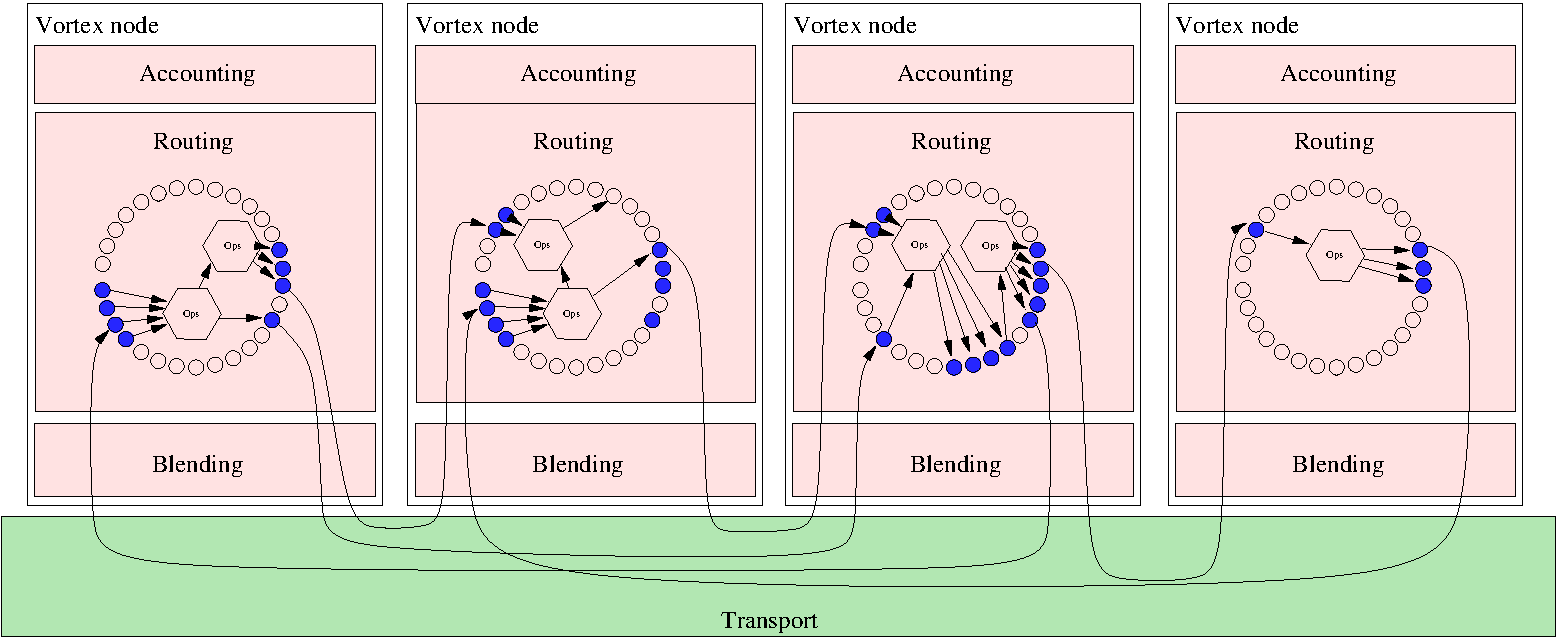
\includegraphics[width=0.6\textwidth,height=90pt]{../../inc/roughProtocolDesign}
	\caption{A rough protocol outline of the MessageVortex protocol}
	\label{fig:protocolLayers}
\end{figure*}

We were unable to identify a protocol withstanding the strong definition of our adversary. We have, however, found many protocols dealing with anonymity and very few dealing with censorship circumventions. We considered these approaches and integrated appropriate techniques in our work. It has to be said, however, that very little of the mentioned protocols here had ever experienced broad adoption. Even more, most of them were never implemented or challenged. 

In terms of censorship circumvention, we found that only a little work has been done in academia. Several technical ways have been explored to circumvent censorship. All of them seem to boil down to the following main ideas:
\begin{itemize}
	\item \emph{Hide data}\\*
	The most common approaches we have found were either mimicking protocols (as in \cite{mohajeri2013skypemorph}), use protocols as payload transports (e.g., \cite{AthanRAM07}) or employ steganography (as in \cite{f5}) or comparable technologies as side channels.
	\item \emph{Copy or distribute data to a vast amount of places in order to improve the lifespan of data}\\*
	This has been done by systems like \cite{freenet}, or WikiLeaks.
	\item \emph{Outcurve censorship measurements}\\*
	Censorship measurements, especially regarding the Internet censorship of China, have been analyzed in depth under technological, sociological and economical aspects (e.g., \cite{Ensafi_2015}, \cite{Clayton_2006}, or \cite{lowe2007great}).
\end{itemize}

For Anonymization the ideas seem mainly to concentrate around onionizing (ToR\cite{tor-spec}, SOR\cite{Egners_2012}, DUO-Onions and Hydra-Onions\cite{iwanik2005duo}), DC networks (DC-Nets\cite{chaum-dc}, Tarzan\cite{tarzan:ccs02}, GAS\cite{AthanRAM07}), mixing (Babel\cite{babel}, MorphMix\cite{morphmix:wpes2002}, Mixminion\cite{minion-design}, Salsa\cite{Salsa}), and distributed hash tables (DHT; e.g., Bifrost\cite{Kondo2009}, BitBlender\cite{Bauer_2008}).

As we use alien transport protocols instead of our protocol, we decided to go for a mixing approach. This approach minimizes the number of messages between the nodes. Furthermore, mixing allows using the nodes in a structureless way as opposed to DC-nets, where we would have to build fixed or ad-hoc rings for exchanging messages. % Unlike other protocols, we do not rely on the logic of mixing on the routing node but entirely on the RBB. Routing nodes follow an onionized set of instructions to build messages. 

\section{The MessageVortex Protocol\label{sec:protocol}}
% In this section, we introduce a new consistent, transport-independent model for representing the different protocols used by MessageVortex. The focus of the description lies in academic concepts. For more technical information specifying the protocol as implemented, refer to \ifCLASSOPTIONpeerreview\cite{Blinded}\else \cite{MessageVortexRFC}\fi. This document provides details such as specific ASN.1 structures outlining every single block.

\subsection{General Design}

Generally, the Vortex System consists only of nodes, whereas a node may be any system always connected to the Internet. This applies to any device regardless of NAT or similar technologies which usually oppose problems for services. Figure~\ref{fig:protocolLayers} shows a network of four nodes passing messages between them. The symbols within the routing layer show the content of a workspace of one ephemeral identity. We elaborate on those two concepts further in the next sections. 

The transport layer is a common message-passing protocol on the Internet. The infrastructure for this message-passing protocol is used in unmodified form by VotexNodes, as it serves as a store-and-forward infrastructure. Although we used SMTP for our experiments, it is not limited to this protocol. The RFC draft document also specifies XMPP. We refer to the upper part of each node as VortexNode. These nodes may be any device with a permanent connection to the Internet (e.g., a RaspberryPi computer or a mobile phone). The message paths shown in the figure are not relevant. Any path layout such as cyclical or tree-like may be possible.

The Vortex system routes messages from a sender to one or more recipients. We refer to the message sent by the sender and received by the recipients as ``message''. We use the term ``VortexMessage'' for the messages exchanged between the nodes containing either message parts, full messages or decoy traffic.

Each VortexNode constitutes out of three layers. A blending layer embedding and extracting messages from the transport layer, a routing layer processing the VortexMessages and providing ``workspaces'' for ``ephemeral identities'', and an accounting layer authorizing messages. We describe the inner workings of these layer in detail in the next sections.

The protocol handles messages which are passed by a transport protocol from node to node. The instructions how and when to pass a message is generated by a node we refer to as ``routing block builder'' (RBB). The RBB defines the path of the message, the type of hiding (blending) in the transport protocol, and the operations applied to each part of the message in each node. To avoid collision of operations, an RBB has on each used node ``ephemeral identities'' with an assigned workspace within the node. Ephemeral identities are short term identities containing a workspace and message quotas for a limited time. Ephemeral identities of a node are unrelated to each other. In the workspaces attached to the ephemeral identities, messages may be assembled, transformed, or decomposed with the operations above. Results are sent to other nodes. Due to the nature of the operations, all messages passed on may be decoy traffic or ``real message parts'' (We prove this claim in section \ref{sec:staticAnalysis}). A node identifies a message destined for it when a message processes data to ID 0 of the identities workspace.

The RBB may be the sender of a block or a different VortexNode. If the RBB is not identical to the sender, then the sender is using the routing block for sending a message without knowing its final destination.

\subsubsection{Message Outline\label{sec:messageOutline}}
%%%%%%%%%%%%%%%%%%%%%%%%%%%%%%%%%%%%%%%%%%%%%%%%%%%%%%%%%%%%%%%%%%%%%%%%%%%%%%%%%%%%
%%% Manual float placement
%%%%%%%%%%%%%%%%%%%%%%%%%%%%%%%%%%%%%%%%%%%%%%%%%%%%%%%%%%%%%%%%%%%%%%%%%%%%%%%%%%%%
\begin{figure*}[ht]
	\centering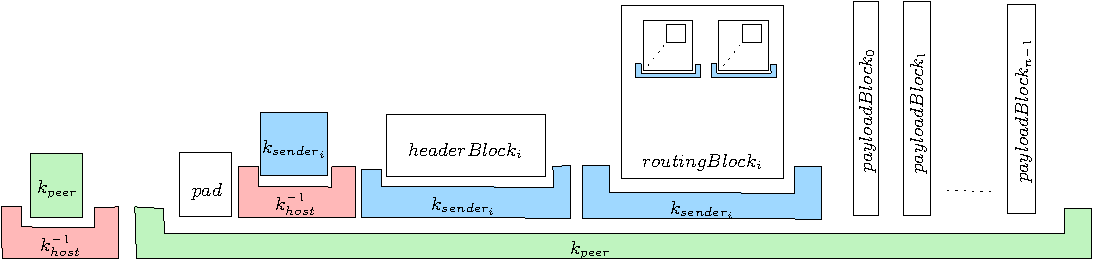
\includegraphics[width=0.6\textwidth]{../../inc/blockLayoutSimplified}
	\caption{A simplified message outline for a message destined for a host $o$}
	\label{fig:messageOutline}
\end{figure*}

%A VortexMessage is passed from one router to another and is embedded as binary data in the transfer protocol. 

Every Vortex node may decide for itself on the support of algorithms and embedding mechanisms. A VortexMessage contains an encrypted symmetric key $E^{host_o}\left(K_{peer_o}\right)$ immediately followed by an inner message $E^{K_{peer_o}}$ which is encrypted with this key. The inner message contains a series of blocks encoded in ASN.1. We show in Figure~\ref{fig:messageOutline} a simplified view on a VortexMessage. The block structure of a Vortex message is as follows:
\begin{itemize}
	\item \emph{Encrypted peer key $K_{peer_o}$}\\*
	Contains the symmetrical key for decryption of follow up header information and payload blocks. The symmetric key is encrypted with the receiving host's public key (i.e. $E^{K_{host_o}}\left(K_{peer_o}\right)$ ). The key $K_{peer_o}$ is known to the RBB, the message sending node, and the message receiving node.
	\item \emph{Padding $PAD$}\\*
	This padding is a defined excerpt of the transferred payload blocks (see further down). It makes sure that the message part encrypted with the peer key does look different for each payload even when reusing keys. This case is not recommended but unavoidable in the case of a reused routing block. Using a different IV is not an option as the IV would be replayed as well.
	\item header block encrypted with $K_{sender_o}$ and signed with the identities private key (detached signature).
	\begin{itemize}
		\item \emph{Identity}\\*
		Authenticated by a signature. It serves as an identifier for the workspace.
		\item \emph{Replay protection information}\\*
		Allows a node to identify replayed messages even if the payload has been modified.
		\item \emph{Forward secret information ($forwardSecret$)}\\*
		Allows a node to identify VortexMessages where tampering occurred by recombining blocks of multiple messages.      
		\item \emph{(optionally) Proof-of-work information}\\*
		Allows a sending node to fulfill a proof of work requirement raised due to a previously sent request. Proof-of-work (puzzle) is required to assign a ``cost'' to a creator of an ephemeral identity. A node fulfilling a puzzle is ``prepaying'' the costs for one or multiple potential message transfers. 
	\end{itemize}
	\item \emph{Routing blocks (encrypted with sender key)}
	\begin{itemize}
		\item \emph{Next hop timing instructions}\\*
		Specifies relative block in time for the building instructions to be carried out. There may be multiple timing instructions. Each of the instructions refers to precisely one routing and one header block.
		\item \emph{Next-hop routing blocks}\\*
		These with $K_{sender_{o+1}}$ preencrypted routing blocks are placed into the VortexMessage created according to the build instructions. They are not readable for the current node.
		\item \emph{Next hop header (encrypted with $K_{sender_{o+1}}$)}\\*
		These preencrypted header blocks are placed into the VortexMessage created according to the build instructions.
		\item \emph{Message build instructions}\\*
		These instructions form the core for the workspace and contain all instructions and the information which payload blocks should be included in each of the messages.
		\item \emph{Next hop peer key $K_{peer_{o+1}}$}\\*
		This part contains one or more peer keys.
		\item \emph{Next hop blending instructions}\\*
		These contain the information about what transport to use, what blending to use, and the address of the next router node.
	\end{itemize}
	\item \emph{Encrypted payload blocks (encrypted with peer key)}
	\begin{itemize}
		\item \emph{Payload blocks}
	\end{itemize}
\end{itemize}

It is important to note that there are two symmetrical keys involved in encrypting and decrypting message headers. Having two keys is not a flaw in the protocol but necessary. 

The first key of a VortexMessage is the peer key $K_{sender_o}$. This key is only accessible with the private key of the node receiving the message and is furthermore known by the RBB. It allows decryption of the routing blocks concerning the current node and the header information. The sender of a message block is therefore not able to tell if a VortexMessage contains one or more routing blocks for the next node. It is important to note that no other node should have access to this information as this builds the unlinkability between two non-adjacent nodes. 

The second key is the peer key $K_{peer_o}$ preceding the encrypted $\mathbf{HEAD}$ block. The RBB chooses the key. This key protects the inner structure of the message. It makes it impossible for any node except the sending or the receiving peer node to detect the inner structure of the message. Without this key, any independent observer with knowledge about the blending capabilities of a receiving node may:
\begin{itemize}
	\item \emph{Easier identify the block structure}\\*
	This remains the case regardless of whether ASN.1 or length prefixed structures are used. If the structure of a vortex Message is identifiable, the messages may be logged or dropped by an adversary.
	\item \emph{Identify the routing block size}\\*
	The value of this information is only minimal as it only reflects the complexity of the remaining routing information indirectly.
	\item \emph{Identify the number of payload blocks and their respective sizes}\\*
	This is valuable information when following the traffic of a message.
\end{itemize}

Furthermore, by providing a pre-encrypted key, we hide the asymmetric key required to the next node. So, a node can compile a message for another node without being aware of the required public key.

\subsubsection{Accounting Layer}
The Accounting layer maintains all local identities called ephemeral identities and controls the overall load to the system. Ephemeral identities are temporary accounting objects identified with the public part of an asymmetric key. 

The accounting layer processes requests from other nodes. Each request is either a request for information about the node, the creation of a new ephemeral identity, or a request to process messages. The accounting layer creates replies to such requests and maintains the accounting information of such an entity. The accounting layer has the options to either accept a request, reject a request, silently drop a request (usually done to improve privacy), or to request the solving of a proof-of-work puzzle (puzzle). To send a reply to the unknown requester, the header block contains a routing block prebuilt by the RBB.

The only implemented puzzle so far is a hash-based puzzle. The puzzle opposes that a header block $\mathbf{H_{t-1}}$ has to be resent including a challenge $c$ (an ASN.1 octet string) and has to result in a specific bit sequence $s$ of the hashed block with signature.

Therefore we assume that a validly solved puzzle when:
\begin{eqnarray}
\mathbf{HEAD}&= D^{K_{sender}}\left(\mathbf{H}\right) = \langle \mathbf{H_{t-1}}, c\rangle\\
puzzleSolved&= H_{spec}(\mathbf{H}).startsWith(s)
\end{eqnarray}

The puzzle has an assigned lifetime. To solve the puzzle successfully, the requesting host has to solve this puzzle within the specified time frame. 

In general, each message is first pre-authenticated by the blending layer (incoming and outgoing). On an incoming, valid message (all decryption successful and all $forwardSecret$ do match), the following checks are executed:



\subsubsection{Routing Layer}
The routing layer processes the messages. Incoming messages are passed after extraction by the blending layer to the routing layer. There the message is disassembled in its components.

As operations, we use some general capabilities such as splitting a message into two payload blocks and merging them again. Another type of operation is encryption and decryption of payload blocks. The third and most important type of operation is a redundancy operation. This operation uses a Reed-Solomon\cite{reed1960polynomial} function to add redundancy information to the data while obfuscating its content. This function has previously been proposed mainly for information sharing systems (e.g., \cite{mceliece1981sharing}).

A routing block may be used once or multiple times if flagged accordingly. Repeating a routing block allows a sender to use a routing block as an anonymous endpoint address. It is essential to understand that reusing a routing block does have downsides in terms of privacy. Reusing a routing block does typically create the same pattern on the network assuming the same workspace layout. While the timing might vary the number of messages and the sequence of messages remains the same. For a full list of weaknesses when reusing routing blocks, see \ref{sec:dynamicAnalysis}.

Tasks of the routing layer are:
\begin{itemize}
	\item Build structure representing the block building and the appropriate block IDs.
	\item Schedule all routing blocks for processing in a priority queue.
	\item Authorize all routing blocks ready for processing with the calculated block sizes.
	\item Process blocks.
	\item Send prepared building blocks to the Blending layer.
\end{itemize}

The workspace of an ephemeral identity is shown in Figure~\ref{fig:workspace}.

\begin{figure}[ht]
	\centering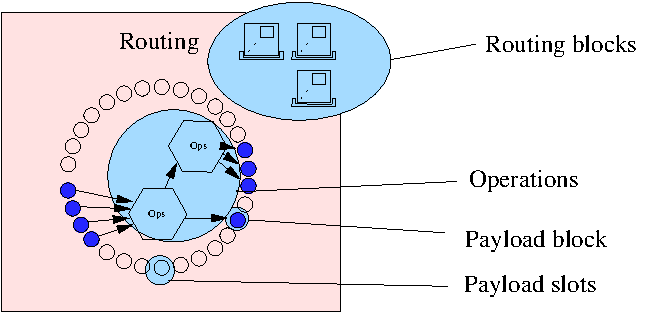
\includegraphics[width=0.6\columnwidth]{../../inc/roughProtocolDesign_workspace}
	\caption{Layout of a workspace}
	\label{fig:workspace}
\end{figure}

Each workspace stores objects for a specific ephemeral identity for a limited amount of time. The workspace receives routing blocks, payload blocks, and operations of the respective ephemeral identity. The lifetime of these objects is either limited by the lifetime of the header block (this applies to payload blocks and operations), or by the routing block (applies to the routing block). As soon as a routing block is due he takes compiles a list of all payload blocks which have to be sent and executes the operations to generate them. The routing layer then assembles the inner message with padding ($\mathbf{PAD}$), the header block with a prefix, the routing block, and the generated payload blocks and encrypts the whole stream with the peer key $K_{peer_{o+1}}$. The header and routing blocks are already pre-encrypted with $K_{sender_{o+1}}$.

\subsubsection{Blending Layer}
The blending layer provides the ``undetectability'' feature of the Vortex system. To avoid transport protocol misuse and unintentional exit nodes of the protocol, the RBB has no control over the transported content except for the hidden VortexMessage and how it is embedded. This rule loads the burden of sensible cleartext payload generation to the blending layer. 

A blending layer may provide multiple strategies to embed a message. In our prototype, we always sent a VortexMessage by embedding its content into an attachment. While F5\cite{f5} is currently preferred for embedding, current implementation supports as well so-called plain embedding simply replacing the file content of the attachment with the VortexMessage. This may be done starting at character 0 or any offset supported by the blending layer (to leave header data intact).

Furthermore, this layer is taking care of multiple problems:
\begin{itemize}
	\item \emph{Translating the message into the transport format}\\*
	This translation includes jobs such as embedding a message as encoded text, as a binary attachment or hide it within a message using steganography.
	\item \emph{Extract incoming messages from the transport protocol}\\*
	Identify incoming messages containing a possible block and extract it from the message.
	\item \emph{Do housekeeping on the storage layer}\\*
	Access protocols may require message deletion.
\end{itemize}

We define the blending layer to work as follows when receiving messages:
\begin{enumerate}
	\item Log arrival time (in UTC) on the transport layer.
	\item Extract possible blocks.
	\item Apply decryption on a suspected header block.
	\item Validate the header using the accounting layer.
	\item Process header requests (if any)
	\item Extract and decrypt subsequent blocks.
	\item Pass extracted blocks and information to the routing layer.
\end{enumerate}

We define the blending layer to work as follows for sending messages:
\begin{enumerate}
	\item Assemble message as passed on by the routing layer.
	\item Using the blending method specified in the routing block build an empty message. 
	\item Create a message body content.
	\item Send the message to the appropriate recipient using the transport layer protocol.
\end{enumerate}

%For our first tests, we used a custom transport layer, allowing us to monitor all traffic quickly, and build structures in a very flexible way. This transport layer works locally with a minimum amount of work for setup and deployment. It furthermore works across multiple hosts in a broadcast domain. The API may be used to support almost any kind of transport layer. After that, we focused on the protocols identified as suitable as transport protocols:
%\begin{itemize}
%	\item SMTP
%	\item XMPP
%\end{itemize}
For the prototype, we have implemented an SMTP transport agent and the respective blending layer.

The routing layer receives the message blocks in a decrypted and authorized form from the blending layer. The routing layer then assembles all information of identity and executes the accepted operations using the available data. 

It is relatively easy to generate a credible cleartext message to pass an automated testing engine. This statement may be verified by looking at the effectivity of today's junk mail filters. These filters have huge problems continuously adapting to the new types of unsolicited bulk emails (UBE).

Things do, however, drastically change if taking a human censor into account. A human censor is not only able to analyze the text and layout of a message. He is furthermore capable of judging on the stringency of a communication. He may deduce data such as relationship and type of writing. Then, he may detect anomalies within conversations and judge whether the communication pattern is more likely to be from a human or a chatbot.

\subsubsection{Applied Steganography and the Dead Parrot}
A human censor can take very complex information into account when it comes to analyses of message content. He is not only able to analyze a message for its content, but he may also see the message in the context of other messages. In \cite{oakland2013-parrot} is expressed that it is easy for a human to determine decoy traffic as the content is easily identifiable as generated content. While this is true for the very general case, there is a possibility here to generate ``human-like'' data traffic to a certain extent. As an adversary may not assume that his messages are replied to, the problem does not boil down to a Turing test. It remains on the level of a ``passive observer Turing test'', in this scenario the censor is only able to judge on the given messages instead of introducing his questions, wordings, and verbal challenges. By enabling the potential nodes to choose their messages and the replies generated to them, we enabled them to choose very reduced types of communications. The chosen messages may even be identifiable as automated messages. 

The most straightforward approach would have been to give a routing block builder the possibility of controlling the decoy message content. While such a possibility would be easy, it would enable a routing block builder to use the node as a ``exit node'' from the system. Blackmailing messages could be sent through the system to a non-participating member and leak at the same time the presence of a routing node. To deny this possibility, we shifted the ability to the routing node.

The VortexMessage itself is binary, and as such, there are only limited possibilities to hide it within the transport protocol. We decided to use attachments or attachment-like structures. Within the attachments, we currently support two types of embedding: plain and steganographic embedding. Plain embedding means that we insert a sequence of blocks into a standard message. This is typically done within files with a weaker structure and high entropy (such as an MP3 encoded file). While this is very hard to detect for a machine, it becomes immediately suspicious for a human censor. A human censor would detect the presence of a payload which does not make any sense.

For steganographic embedding, we decided to go for F5\cite{f5}. It is a reasonably well-researched algorithm which attracted many researchers. The original F5 implementation had a detectable issue with artifacts\cite{F5broken} caused by the recompression of the image. This issue was caused only due to an issue in the reference implementation, and the researchers have provided a corrected reference implementation without the weakness. %Like always, the type of embedding may be specified and replaced upon request. 

\subsection{The Core: Operations Executed in a Workspace}
We differentiate three types of operations:
\begin{itemize}
	\item Splitting and merging of chunks
	\item Encryption and decryption of chunks
	\item Redundancy calculations carried out on chunks
\end{itemize}

The first two Operations do not provide a high level of unlinkability as they do allow analysis such as hotspot analysis and produce continuously inclining, steady or declining message sizes depending on the type of use. The third operation, however, adds a whole lot of new possibilities in conjunction with the other two.

\subsubsection{Splitting and Merging}
The $splitPayload$ operation splits a payload block into two chunks of different or equal sizes. The parameters for this operation are:
\begin{itemize}
	\item Source payload block $pb_1$
	\item Fraction $0<f<1$ of $pb_1$ transferred to the first chunk $pb_2$
\end{itemize}

If $len(pb_1)$ expresses the size of a payload block called $pb_1$ in bytes, then the two resulting blocks of the SpitPayload Operation $pb_2$ and $pb_3$ have to follow the following rules:
\begin{eqnarray}
split(f, pb_1) & = &\langle pb_2, pb_3 \rangle\\
pb_1.startsWith(pb_2)\\
pb_1.endsWith(pb_3)\\
len(pb_2) & = & \lfloor len(pb_1)\cdot f\rfloor\\
len(pb_1) & = & len(pb_2) + len(pb_3)
\end{eqnarray}

The $mergePayload$ operation combines two payload blocks into one and is defined as the reversing function to the $splitPayload$ function. 
%
%The parameters for this operation are:
%
%\begin{itemize}
%	\item first source payload block $pb_1$
%	\item second source payload block $pb_2$
%\end{itemize}
%
The $mergePayload$ operation is defined analogous to the splitPayload operation and joins the two blocks into one.
%If $len(pb)$ expresses the size of a payload block called $pb$ in bytes then resulting block of the MergePayload Operation $pb_3$ have to follow the following rules:
%
%\begin{eqnarray}
%merge(pb_1, pb_2) & = & pb_3 \\
%pb_3.startsWith(pb_1)\\
%pb_3.endsWith(pb_2)\\
%len(pb_3) & = & len(pb_1) + len(pb_2)
%\end{eqnarray}

\subsubsection{Encryption and Decryption}
The $encryptPayload$ operation encrypts a payload block $pb_1$ symmetrically resulting in a block $pb_2$. The length of block $pb_2$ may vary according to mode and padding chosen. The parameters for this operation are:
\begin{itemize}
	\item Source payload block $pb_1$
	\item Encryption specification $spec$
	\item Symmetric key $K$
\end{itemize}

The operation follows the following rules (please note section \ref{sec:encNot} for notation):
\begin{eqnarray}
encrypt(pb_1, spec, K_a) & = & pb_2 \\
pb_2 & = & E_{spec}^{K_a}\left( pb_1 \right)\\\
len(pb_2) & \geq & len(pb_1)
\end{eqnarray}


The $decryptPayload$ operation decrypts a payload block $pb_1$ symmetrically resulting in a block $pb_2$. It is defined as the reversing operation to $encryptPayload$. 

%The parameters for this operation are:
%
%\begin{itemize}
%	\item Source payload block $pb_1$
%	\item Decryption specification $spec$
%	\item Symmetric key $K$
%\end{itemize}
%
%The operation follows the following rules (please note section \ref{sec:encNot} for notation):
%\begin{eqnarray}
%decrypt(pb_1, spec, K_a) & = & pb_2 \\
%pb_2 & = & D_{spec}^{K_a}\left( pb_1 \right)\\
%len(pb_2) & \leq & len(pb_1)
%\end{eqnarray}

\subsubsection{Redundancy Operations}
These operations build the core of the mixing operations. The operation allows to add to a message redundancy information or to rebuild a block from a chosen set of information. 

\begin{figure}[ht]\centering
	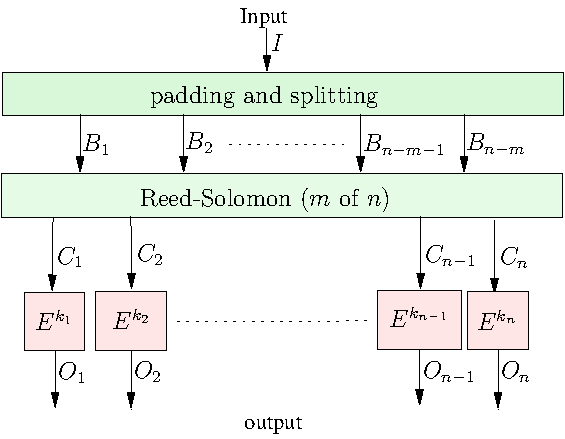
\includegraphics[width=0.5\columnwidth]{../../inc/addRedundancyOp}
	\caption{Outline of the addRedundancy operation}
	\label{fig:addRedundancyOperation}
\end{figure}

The operation itself is shown in Fig.~\ref{fig:addRedundancyOperation} and may be subdivided into the following operations:
\begin{itemize}
	\item Pad the original message block in such a way, that all resulting blocks are a multiple of the block size of the encrypting cipher.
	\item Apply a Reed-Solomon operation in a given GF space with a Vandermonde matrix.
	\item Encrypt all resulting blocks with unpadded, symmetrical encryption.
\end{itemize}

The padding is not standard padding from encryption. The reason for this lies in the properties required in the padding. These properties were:
\begin{itemize}
	\item The padding must not leak whether the rebuild cycle was successful or not.
	\item The padding should not leak whether a removeRedundancy operation was successful or not. 
	\item Anyone knowing the routing block content and the transmitted message must be able to predict any treated block including all padding bytes.
	\item The padding must work with any size padding space.
\end{itemize}

The padded block $\mathbf{X}$ is created from a padding value $p$, the unpadded block $\mathbf{M}$ and a srie of padding bytes. We build $\mathbf{X}$ for a function $RS_{\text{m of n}}$ and an encryption block $\mathbf{M}$ sized $K$ as follows:
\begin{eqnarray}
i          & = & len(\mathbf{M})\\
e          & = & k \cdot n\\
l          & = & \left\lceil\frac{i + 4 + C2 }{e}\right\rceil\cdot e\\
p          & = & i + \left( C1 \cdot l \pmod{\left\lfloor\frac{2^{32}-i}{l}\right\rfloor\cdot l}\right)\\
\mathbf{X} & = & \langle p,\mathbf{M},R_{t}\left(s,l-i-4\right)\rangle
\end{eqnarray}    
The remainder of the input block, up to length $l$, is padded with random data. The random padding data may be specified by RBB though a PRNG spec $t$ and an initial seed value $s$. The message is padded up to size $L$. All resulting, encrypted blocks do not require any padding. This baecause the initial padding guarantees that all resulting blocks are dividable by the block size of the encrypting function. If not provided by an RBB, an additional parameter $C1$ is chosen as random positive integer and $C2=0$  by the node executing the operation.

To reverse a successful message recovery information the of a padded block $\mathbf{X}$, we calculate the original message size by extracting $p$ and doing $len(\mathbf{M})=p \pmod{ len(\mathbf{X})}$.

This padding has many important advantages:
\begin{enumerate}
	\item The padding does not leak if the rebuilding of the original message was successful. Any value in the padding may reflect a valid value.
	\item Since we have a value $C2$, the statement that a message size is within $len(\mathbf{X})<size<(len(\mathbf{X})-k\cdot n)$ is no longer true and any value smaller $len(\mathbf{X})-k\cdot n$ may be correct as well.
	\item An RBB may predict the exact binary image of the padded message when specifying $C1$, $C2$, and $R_{t}(s,)$.
\end{enumerate}

\begin{figure}[ht]\centering
	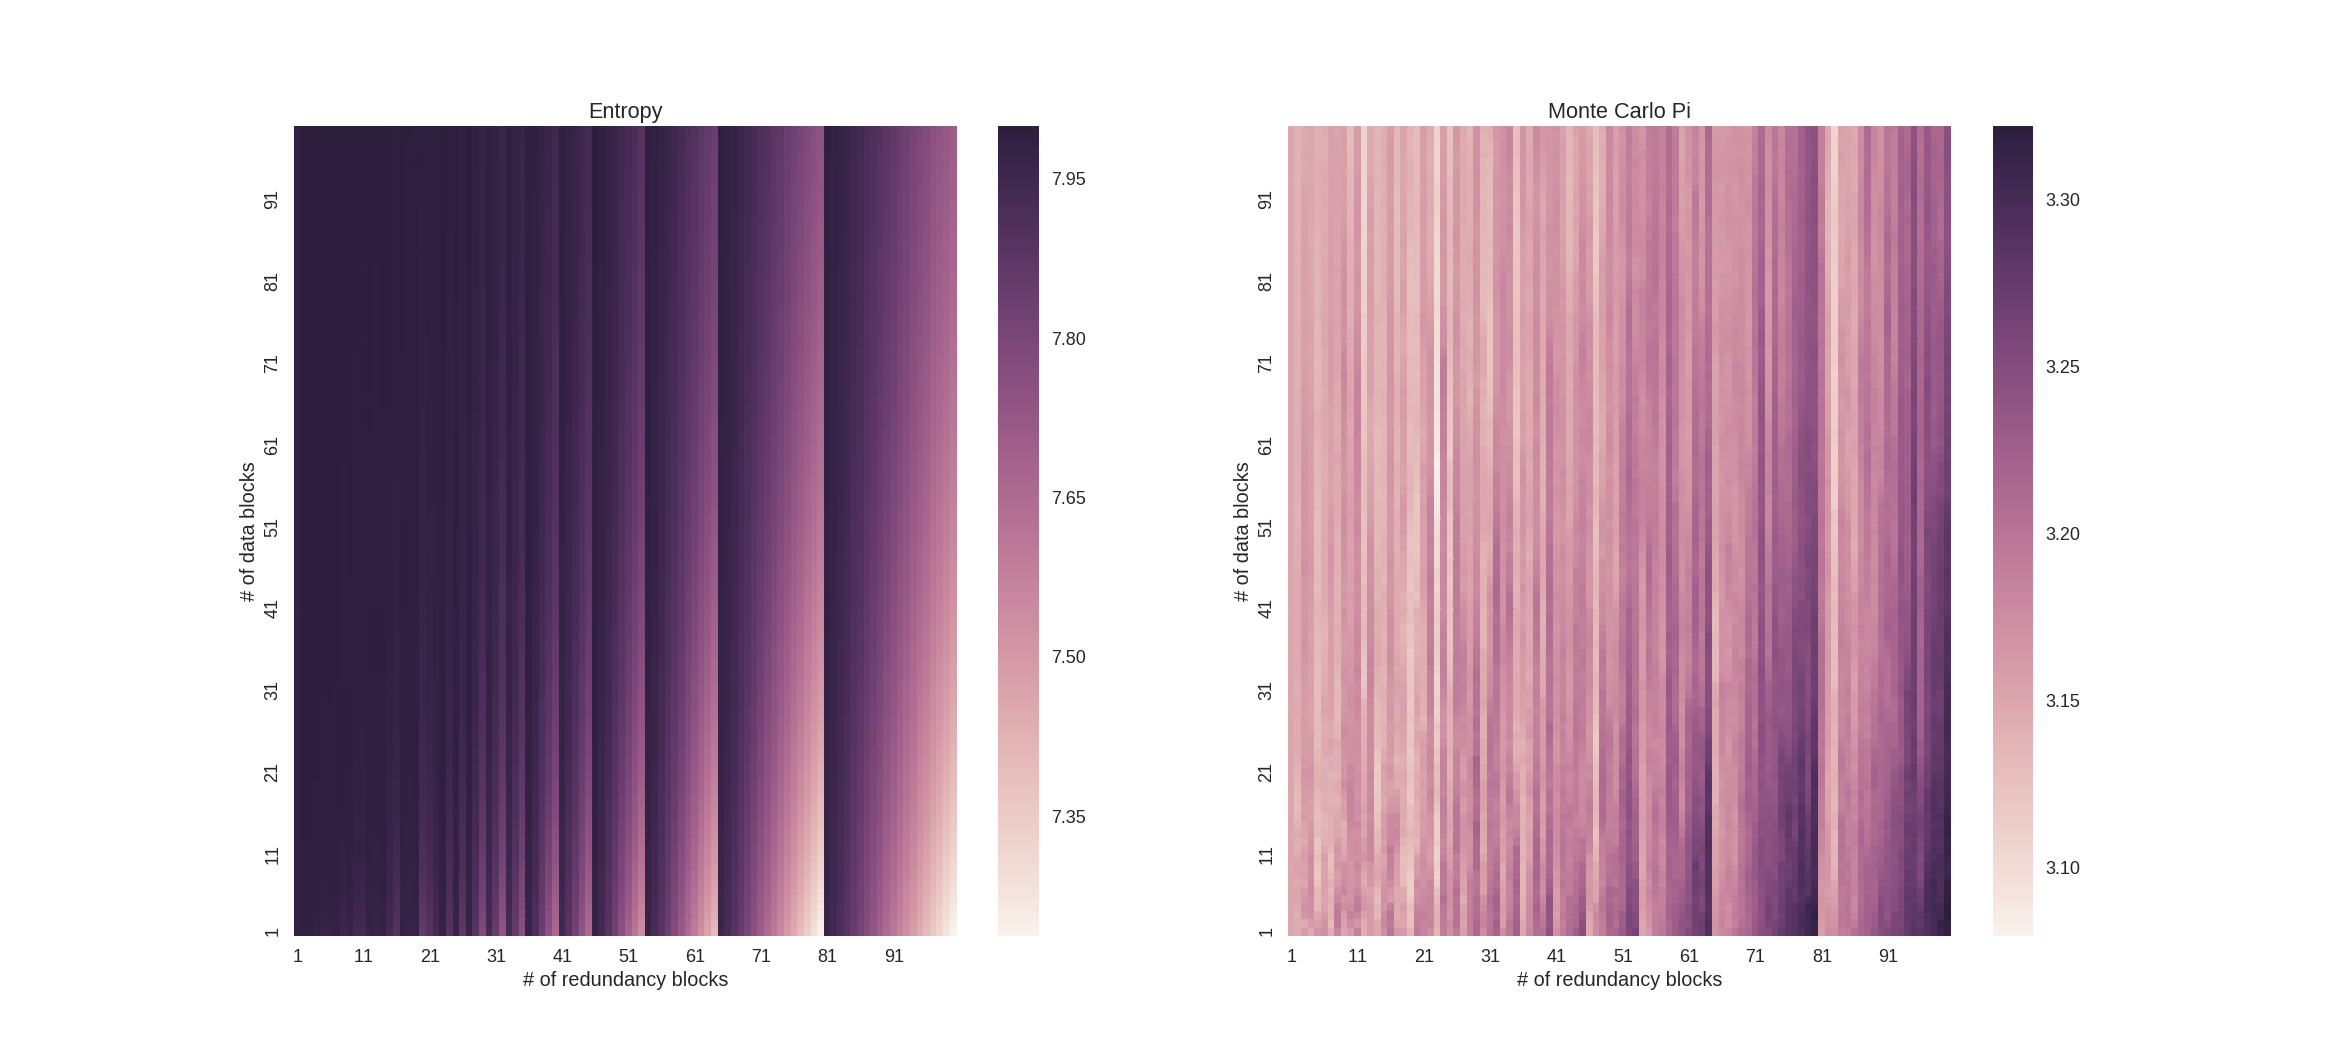
\includegraphics[width=1\columnwidth]{../../inc/randomblock_10kb}
	\caption{Resulting entropy of addRedundancy without encryption step}
	\label{fig:entropy}
\end{figure}


The Reed-Solomon operation is done with a Vandermonde matrix. Unlike in error-correcting systems, we do not normalize the matrix so that the result of the first blocks is equivalent to the original message. Instead, the error-correcting information is equally distributed over all resulting blocks adding further obfuscation. Since the entropy of the resulting blocks is lowered as shown in Fig.~\ref{fig:entropy} and may thus leak an estimate of how a resulting block may have been treated, we added the encryption step to equalize entropy again. The previously introduced padding guarantees that there is no further padding on block level required. The presence of such padding could leak in case of decryption whether the block has been successfully decrypted or not.

\subsection{Usage of the Protocol}
First, a sending node collects either a set of nodes and keys it wants to use and creates identities on these nodes using header requests. Then the sender creates a routing block containing all the routing instructions (hops and operations). Alternatively, a sender may use a premanufactured routing block for the specified target. This routing block is then concatenated to a message and passed to the locally running routing node. From there the message is routed as defined in the routing block. An example of such a route is shown in Figure~\ref{fig:protocolLayers}.

A trivial routing block may only include the direct hop from the sender to the receiver. When adding subsequent decoy paths leaving the receiver, it is even for an adversary capable of mapping ephemeral identities to the respective RBB impossible to tell the final recipient. This since a message may increase or decrease in its size even after the final delivery through the addRedundancy operation. Even the recipient node is unable to tell if there are any other messages routed if appropriately crafted.

If a node is always using a set of $K$ recipients of its address book, at least $K$ anonymity is achieved. If an adversary compromises all other nodes involved in routing, he is still unable to obtain additional knowledge. All outgoing traffic from this node may be related or unrelated to the observed message as linking between messages is no longer possible. Essential properties, such as message size or routing block size, may increase or decrease. If the adversary can monitor all messages from the inner side of the system (all messages are passed by an adversary controlled node to the honest node), he may assume that a routing block, in general, may only decrease in size. Starting from this assumption, he might be able to eliminate some candidates for linking.

\section{Analysis of the MessageVortex Design\label{sec:discussion}}
We first focus on the protocol itself to show the strength an weaknesses of the protocol. After that, we focus on the dynamic part and see what type of data may be collected when considering not only the protocol but the whole message flow. We then present guidelines for different jurisdictional types.

We focus on an adversary in an environment, where the participation as a MessageVortex router, is considered a criminal act and highlight some additional constraints applying in such situations.

\subsection{Static Protocol Analysis\label{sec:staticAnalysis}}
A VortexMessage is not identifiable as the message is structureless on the outside. The VortexMessage itself follows the encrypted key without any structure. Therefore, we require the hosts private key to tell whether there is VortexMessage within a transport message or not.

The communication itself is undetectable for an adversary only observing as long as the blending mechanism is secure, and the plain text communication of a node does not differ from any other communication. While we can monitor the first criteria, the latter is far harder to achieve or measure as it involves many unobvious properties. Obvious properties are the credibility of message content or stringency of communication over all messages. Unobvious properties may be the frequency of messages (e.g., bundling of messages showing an inappropriate speed of writing to a single entity or 24x7 activity of a natural person) or a message exchange massively in favor of one recipient. We were not able to create a set of measurable properties covering these properties.

The padding block $PAD$ makes sure that, even if a routing block is reused, the VortexMessage structure is not the same. However, the preceding block with the key remains the same unless the RBB provided multiple key blocks. If a key block is reused, an adversary to identify repeated MURBs by this fingerprint.


Next, and one of the biggest problems we found is that a VortexNode is aware of its immediate peers. This flaw is because we do require a routable address for the transport protocol. Vortex nodes may thus discover their immediate peers. It is, on the other side, not possible to use discovered peers. If an adversary wants to use a peer, a transport address and a host key are required. A VortexNode may query this key, but there is no obligation to reply for the node asked for the key. We were unable to find a protocol commonly used on the Internet, allowing to cloak the receiving node of a message.

An active adversary may not create its routing blocks or header blocks and inject them due to the forward secret. He may, however, replace the peer key of a message. As this key is known to him, he gains no additional knowledge. Replacing the sender key block breaks the message. Replacing the header or routing block of the message with another header or routing block from the same ephemeral identity breaks the message unless the RBB reused the sender key and the forward secret. Finally, exchanging, omitting, or adding payload blocks renders the message inoperable, but does not generate additional knowledge. Replying the same or a modified block does not generate any pattern on the network as the replay protection stops propagating messages at the next node. Thus, a replayed block does not generate new knowledge to an observer.

All operations may apply to true message chunks as well as decoy traffic. As a node cannot tell if a traffic arriving is a decoy or true message content, it is unable to tell apart what outgoing traffic is a decoy. An encrypted block is of the same nature before and after encryption. As we do not know the blocks nature before, we are unable to tell the blocks nature after the encryption. The same argument applies to decryption, split, and merge operations. 

Redundancy operations are alike. They, however, fulfill an additional purpose. A $addRedundancy$ operation adds size to a message without differentiating between redundancy information and original payload. If the original block was a decoy, then all resulting blocks are decoys. If an originating block was message content, then all resulting blocks hold the same amount of data from the original block. So, this operation allows decoy traffic generation without enabling a generating node to identify the decoy traffic.

\subsubsection{Endpoint Operation}
Depending on the blending method, an adversary may identify single messages as long as they are detectable. Detectability depends on various factors, such as (broken) file structure, uncommon attributes (e.g., mismatching entropy), unrelated message flow (e.g., \cite{oakland2013-parrot}), or non-human behavior (e.g., message traffic 24x7)
% If an adversary identifies an endpoint successfully, then all peering endpoints of the same protocol may be identified as well by following the message flow. This does, however, not enable an adversary to inject messages as the host key $K_{host_o}$ is not known. 

Assuming a global observer as an adversary and unencrypted traffic, he might discover the originating routing layer and thus identify it as Vortex node by following traces of the transport layer. In most protocols, however, this address is spoofable and not a reliable source for the originating account.

\subsubsection{Conclusions Based on Ephemeral Identities}
The knowledge a node may gain from ephemeral identities is minimal. The ephemeral identity is created by a node unknown to the receiver of the request. The only thing we know is what node was adjacent when creating the ephemeral identity. As the creation of an ephemeral identity is not linked to any other identity or ephemeral identity relationship between ephemeral identities on two nodes cannot be established. If two adjacent nodes cooperate when processing two linked ephemeral identities, no additional knowledge may be won. If two collaborating nodes have one or more non-collaborating nodes between them, they lose all linking knowledge due to the non-collaborating nodes. 

\subsubsection{Conclusions from Operations}
Operations have been carefully crafted to leak as little information as possible. Being able to encrypt or decrypt a payload block does not leak any information. The data processed may be true message traffic or decoy as we do not know what the nature of the received message was. If an RBB avoids repeating patterns of blocks on nodes, it is not possible to link ephemeral identities of two non-adjacent nodes. 
%Repeating patterns may arise, for example, if a block $pb_1$ is decrypted and re-encrypted on two nodes. In this case, both nodes may match the message as it contains the same content between the operations.

%\begin{eqnarray*}
%	\text{node f:}\\
%	& pb_2 & = D(pb_1\\
%	& pb_3 & = E^{K_t}(pb_2)\\
%	\text{node f+1:}\\
%	&.\\
%	&.\\    
%	\text{node f+x:}\\
%	& pb_4 & = D^{K_t}(pb_3)\\
%\end{eqnarray*}
%
In this example the patterns of $pb3$ and $pb_4=pb_2$ are two patterns repeating on non-adjacent nodes. The same conclusions are even more valid for splitting operations. These two operations should be regarded as helpers for the $addRedundancy$ and $removeRedundancy$ operations. These operations may be used to generate decoy traffic or to destroy data without knowledge of doing so of the processing node. If we process a function $addRedundancy_{2 of 3}$ any of the output blocks contains the input payload and any two of them may be used to recover the data. At the same time, an operation $removeRedundancy_{2 of 3}$ may be successful or not. The node is unable to differentiate between the two states. The padding applied and the unpadded encryption makes it impossible to judge upon success or fail of an operation.

\subsubsection{Ill-behaving Nodes and Unlinkability}
As the communication pattern is defined by the RBB and not always the same, it is hard to judge on the security. We may, however, look at some generic examples and show that we can achieve the goals byzantine fault tolerance, privacy and unlinkability, and anonymity. Figure~\ref{fig:messagePaths} shows a sending node $s$, a series of routing nodes $n_i,j$ assembled to routing chains. Furthermore, we have a $r$ for which the message is destined and a set of nodes $a_k$ building the anonymity set. Neither the number of chains $j$ nor the length of the chains $i$ is relevant. We furthermore have to keep in mind that we trust sender $s$ and receiver $r$. Any possible routing block may be reduced to this scheme if knowing the exact building instructions applied by the RBB.
%%%%%%%%%%%%%%%%%%%%%%%%%%%%%%%%%%%%%%%%%%%%%%%%%%%%%%%%%%%%%%%%%%%%%%%%%%%%%%%%%%%%
%%% Manual float placement
%%%%%%%%%%%%%%%%%%%%%%%%%%%%%%%%%%%%%%%%%%%%%%%%%%%%%%%%%%%%%%%%%%%%%%%%%%%%%%%%%%%%
\begin{figure}[ht]
	\centering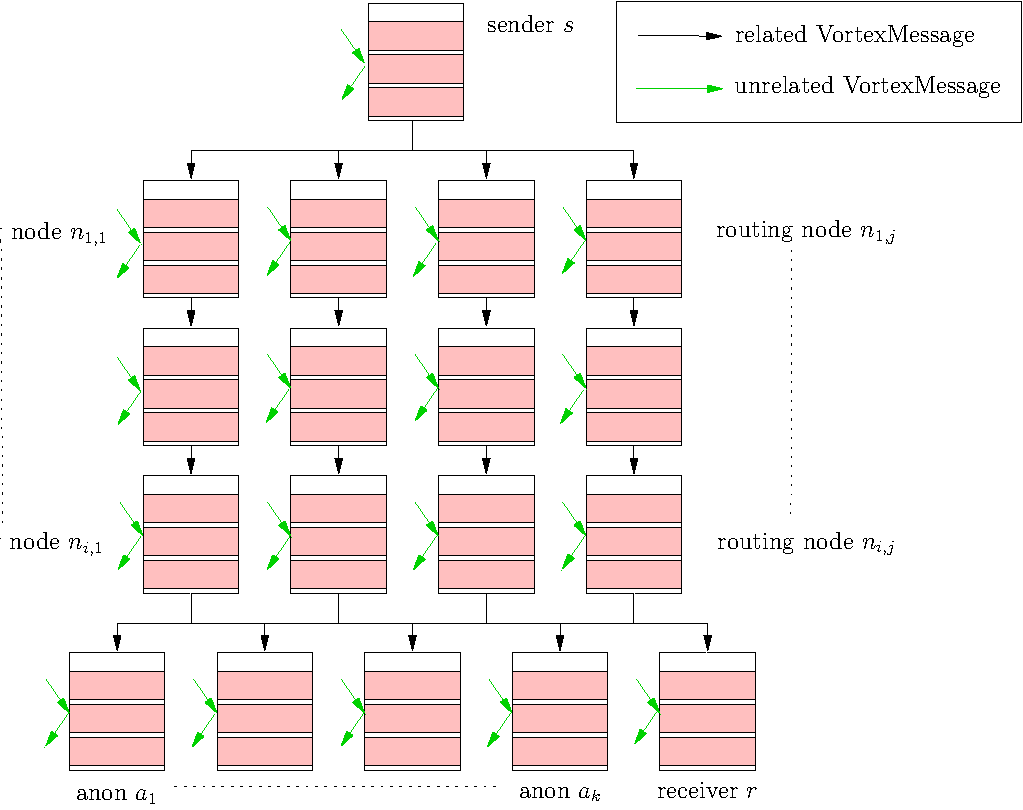
\includegraphics[width=0.5\columnwidth]{../../inc/messagePaths}
	\caption{A possible path of a VortexMessage}
	\label{fig:messagePaths}
\end{figure}

We have to consider the fact that two adjacent nodes collaborating may build one combined workspace executing all operations. They are, therefore, able to link all operations of these two adjacent nodes and follow all incoming and outgoing paths. We, therefore, may assume that two adjacent nodes or an uninterrupted series of collaborating nodes may be substituted by one node.

So a routing node $n_{1,}$ may not know if a VortexMessage received from $s$ is the result of processing another message or the message has been injected on node $s$. Furthermore, if $s$ was acting as a routing node, it successfully unlinked the message from any previous node. The sending node $s$ may send a message by first employing an $addRedundancy$ operation or splitting and encrypting the message. Each path through the streams has then not enough information to rebuild the combined message. If employing an $addRedundancy$ operation, a receiver $r$ may recover a message, if sufficient paths through the routing nodes were acting according to the protocol. Paths with misbehaving nodes may eventually be identified depending on the number of redundancy operations. Assuming that the RBB included proper padding Information for the receiver $r$, the receiver may identify what set of VortexMessages leads to the original message due to the padding applied before the $RS$ function. So if sufficient paths, depending on the chosen operations at $r$, provide correct data, we may recover nodes misbehaving in our paths. If one node in a path is not collaborating with adjacent nodes in the path, the path of the Vortex Message becomes unlinked as previously shown with sender $s$. If multiple paths are used, all paths must have at least one honest node to unlink the message. 

If all nodes in the anonymization set $a_1$\ldots$a_k$ are honest, any preceding node may not know whether the message ends at that node or the message is just routed through an honest node. Even if some of the anonymization nodes are not honest or collaborating with an adversary, the anonymity set may be reduced in size, but the receiver is still part of the anonymity set spanning the honest anonymization nodes. So, we have shown that depending on the chosen routing block anonymity, unlinkability, and fault tolerance against a misbehaving node may be achieved. AN RBB may furthermore send additional VortexMessages to suspected misbehaving nodes. If misbehavior is reproducible within an ephemeral identity, the RBB may identify it by picking up parts of the previously sent message and comparing them to an expected state. An RBB may even introduce message paths leading back to the RBB itself. Such a message path may allow observation of progress and success of the message delivery.

\subsection{Dynamic Protocol Analysis\label{sec:dynamicAnalysis}}
A global observer is unable to analyze a message flow by timing or pattern of the exchanged packet even when being able to identify message vortex packages. Source and target nodes of a message are indistinguishable from other nodes even if having infiltrated significant portions of the network. Cooperation between adjacent nodes does not gain more information. Linking of the message of two non-adjacent nodes is not possible as there are no linking attributes.

\subsubsection{Bootstrapping of Addresses and Identities}
Using the header requests an adversary may discover nodes over time. While it is not possible to screen traffic destined to such nodes, a global observer may identify peer partners of these nodes on the transport level.

\subsubsection{Discovery of Peer Nodes}
Besides attacking the message content, attacking the routing nodes is an option for an adversary in a jurisdiction where the operation of such a node is a criminal act. 

\subsubsection{Findings based on Adversary Environment}
In environments containing only global observers and no jurisdictional constraints regarding the technology, a VortexNode may disclose its presence. As a result, a VortexNode is not forced to cloak its presence. In such an environment, an RBB should choose the operations to be sensible, but great care is not required. Even if there is a node with a known owner of the node and a suspected message is received, the owner may credibly claim that the message in question was a decoy. No information obtained by any node involved in the routing of the message may proof anything else. Since a message may be split into any number of parts and related messages are only identifiable with a high degree of improbability even meta information such as the real size of the message, the sending time or the involved parties in the anonymity set are unknown. %This statement is still valid if we consider an active adversary.

In environments where using a VortexNode is subject to criminal prosecution, much more care has to be applied. As all routing nodes know their immediate peer, we were only able to find two weak solutions to this problem. The first solution is only to use trusted nodes. If we can trust all routing nodes, no external observer may prove that the message flow is, in fact, MessageVortex traffic. The RBB may reduce the set of uncovered nodes by applying communicating groups of nodes (communication cells) with defined gateways nodes between them. In such a scenario, only a cell and adjacent cells may be discovered.

\subsubsection{Issues When Reusing Routing Blocks}
Reusing a routing block is required if the receiver is not known, and a continuous stream of messages is required. Although it is possible to use multiple single route routing blocks (SURB) instead of one multi-use routing block (MURB), it is costly. These costs arise due to the necessary calculation power to create identities. MURBs do have, however, significant drawbacks in terms of unlinkability and should be, therefore, avoided if possible.

A MURB creates a repeated pattern on the network in terms of messages. For a routing node, it is evident that the same tuple of communication partners is exchanging messages. The size of the VortexMessage allows in such a case an estimate of the current size in relation to the previous messages.

Furthermore, security is affected when using MURBs. A MURB may be replayed and allows thus to exhaust quotas of an ephemeral identity. To counter such exhaustion, the protocol introduces a maximum replay rate, but this is only weak protection.

\section{Conclusion}
Creating a protocol which is possibly censorship-resistant, is already hard. The analysis showed that even when a protocol is crafted with great care, braking unobservability is far simpler than doing it right. MessageVortex does show the desired properties. The protocol allows sending a message from a sender to a recipient without exposing the linking between the two. Traditional analysis, such as hotspot analysis, fail since the operations successfully hide properties of the message flow. At the same time, we were able to present a system which requires an unmatched amount of observation, infrastructure, and calculation power to be broken.

\subsection{The Missing Links and Future Research}
For this protocol to be of any use, a user-friendly implementation is required. The currently released implementation works as a prototype for academic research. It is, however, far beyond from being user-friendly. A new implementation must provide excellent censorship-resistance while providing easy to use recipes for message transfer.  For the traffic to be truly undetectable, chatbots must generate meaningful conversation between blending nodes. This conversation does not necessarily boil down to a Turing test. It is sufficient that two blending layers are capable of setting up communication, which is indistinguishable from a regular human or machine communication. As an adversary is typically not able to generate own traffic without exposing the probing activity and a blender is not required to such probes, an attacker is very limited. Furthermore, some issues have been identified, relating to updating nodes. A node should be able to request the software over VortexMessages as official sources for updates may be blocked. Another exciting field of academic research is creating strategies for Routing block builders (RBB). We currently have a toolset of powerful operations, but academic researched strategies or guidelines for good routing blocks are missing. 

The hardware of a routing node should be protected with a small platform featuring deniable encryption and anti-forensic measures. We are currently investigating the possibility of creating such a cheap platform based on a RaspberryPi Zero.

\subsection{Further Reading}
This paper is a very rough overview of the MessageVortex protocol. For those interested in the technical implementation details the current version of the RFC\cite{MessageVortexRFC}. For a more elaborated analysis covering additional topics such as the blending types, additional literature research, or arguments for a decision, we recommend reading the thesis paper \cite{messageVortex}. In this document, we cover additional details such as elaborated analysis on the protocol, the implications of the connection between transport endpoints and VortexNodes, or an analysis of the plain embedding technique.

\bibliographystyle{ACM-Reference-Format}
%\citestyle{acmauthoryear}

\Urlmuskip=0mu plus 1mu % fixes URL breaks
\bibliography{../../messageVortex}

\end{document}


